\documentclass[tikz,border=10pt]{standalone}
\usepackage{amssymb} % For math symbols if needed

\begin{document}
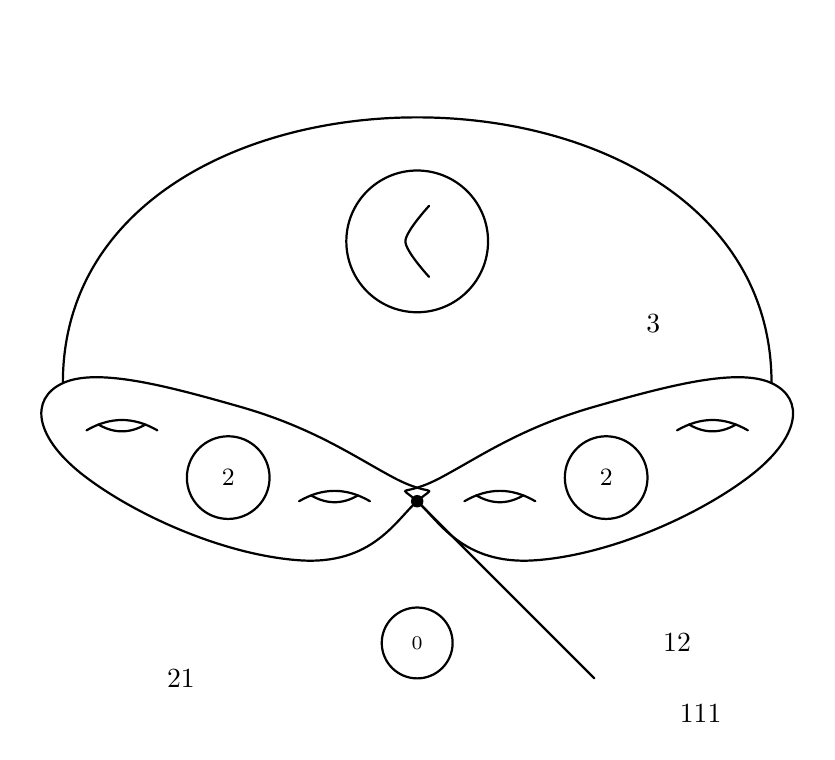
\begin{tikzpicture}[scale=1.5, line width=0.8pt, line cap=round, line join=round]

    % --- 1. Coordinate Definitions ---
    \coordinate (Center) at (0,0);
    \coordinate (LeftTip) at (-3, 0.5);
    \coordinate (RightTip) at (3, 0.5);
    \coordinate (TopCenter) at (0, 2.5);

    % --- 2. The Main "Lobes" (The glasses/infinity shape) ---
    % Left Lobe
    \draw plot [smooth cycle, tension=0.8] coordinates {
        (Center) 
        (-1, -0.5) 
        (-2.8, 0.2) 
        (-3, 1) 
        (-1.5, 0.8) 
        (-0.2, 0.2)
    };

    % Right Lobe
    \draw plot [smooth cycle, tension=0.8] coordinates {
        (Center) 
        (1, -0.5) 
        (2.8, 0.2) 
        (3, 1) 
        (1.5, 0.8) 
        (0.2, 0.2)
    };

    % --- 3. The Large Upper Dome ---
    % Arcs from the far left of the left lobe to the far right of the right lobe
    \draw (-3, 1) .. controls (-3, 4) and (3, 4) .. (3, 1);

    % --- 4. Central Vertex ---
    \fill (Center) circle (1.5pt);

    % --- 5. Internal Circles & Symbols ---

    % Top Circle (Region 1)
    \draw (0, 2.2) circle (0.6);
    % Drawing the squiggle inside (looks like an integral or a '1')
    \draw plot [smooth] coordinates {(0.1, 2.5) (-0.1, 2.2) (0.1, 1.9)};

    % Left Circle (Region 2)
    \draw (-1.6, 0.2) circle (0.35);
    \node at (-1.6, 0.2) {\small 2};

    % Right Circle (Region 2)
    \draw (1.6, 0.2) circle (0.35);
    \node at (1.6, 0.2) {\small 2};

    % Bottom Circle (Region 0 / Spiral)
    \draw (0, -1.2) circle (0.3);
    % Drawing a small spiral/squiggle inside
    \draw (0, -1.2) node {\scriptsize $0$}; % or spiral approximation

    \draw (-2.8,0.6) to[bend left] (-2.2,0.6);
    \draw (-2.7,0.65) to[bend right] (-2.3, 0.65);
    \draw (-1,0) to[bend left] (-0.4,0);
    \draw (-0.9,0.05) to[bend right] (-0.5, 0.05);
    \draw (2.8,0.6) to[bend right] (2.2,0.6);
    \draw (2.7,0.65) to[bend left] (2.3, 0.65);
    \draw (1,0) to[bend right] (0.4,0);
    \draw (0.9,0.05) to[bend left] (0.5, 0.05);
    %\draw (-1.2,-6.4) to[bend right] (1.2,-6.4);

    % --- 6. The Line Segment ---
    % Emanating from center to bottom right
    \draw (Center) -- (1.5, -1.5);

    % --- 7. Labels and Annotations ---


    % Floating "3" inside the dome, right side
    \node at (2, 1.5) {3};

    % "21" Bottom Left
    \node at (-2, -1.5) {21};

    % "12" Bottom Right
    \node at (2.2, -1.2) {12};

    % "111" Bottom Right (below 12)
    \node at (2.4, -1.8) {111};

\end{tikzpicture}
\end{document}